%\section{Neural Networks}
\label{sec:BNN}

Neurons are nerve impulse-conducting cells that shape the nerves, the brain and the spinal column. They are considered as the functional unit of the nervous system. A typical neuron is divided into four regions: the soma or cell body, the axon, the dendrites and the synapses. The next lines try to describe very briefly the main characteristics and functions of each region and how they interact each other \cite{levitan2015neuron}. \figref{neuronstructure} shows how they are organized.

\begin{figure}[!ht]
\centering
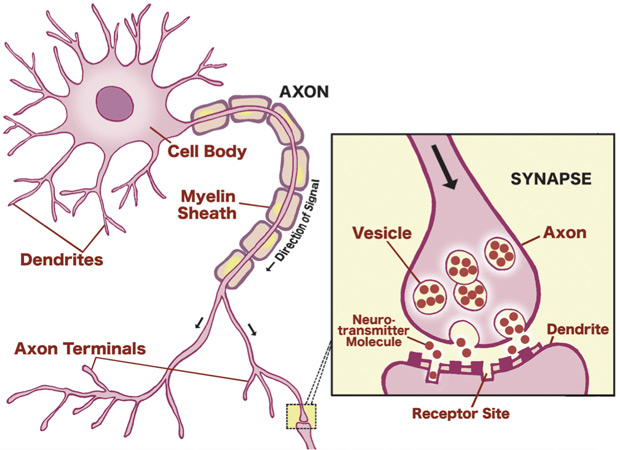
\includegraphics[width=0.6\textwidth]{images/neuronstructure.jpg}
\caption{Model of the structure of a neuron}
\label{fig:neuronstructure}
\end{figure}

The soma is the main part of the neuron in which the dendrites and the axon branch off of. It also contains the cell nucleus.Dendrites are thin structures that extend for hundreds of micrometres and branch multiple times shaping a complex ``dendritic tree''. An axon is a special cellular extension that travels for distances ranging from micrometers to meters before terminating.

The synapses are specialized regions or junctions that allows cell to cell connection for communicating. At the majority of synapses, a neuron receives information from other neurons through its dendrites. In the soma, the input signals are integrated and processed, and the axon is where the output signal is transmitted to a third neuron. This way, neurons can connect to each other to form neural networks.

The information that neurons exchange is electrical in nature, although the process is mediated by chemical substances. 
This way, axons are specialized for the conduction of a particular type of electric impulse called \emph{action potential}.
Then, the transmission of the information to a different neuron is carried out with the help of some biomolecules called neurotransmitters. 
This latter chemical process is called \emph{synapsis}. 
Thus, if a neuron $j$ sends a signal to neuron $i$, the former is called \emph{presynaptic} neuron and the latter is known as the \emph{postsynaptic} neuron. 
It is the arrangement of neurons and the strengths of the individual synapses, determined by the chemical
process of the neurotransmitters, that establishes the function of the neural network.

For the development of some ANNs algorithms, it is important to understand how an action potential is and conducts. We describe its mechanism in the following section.

\subsection{The action potential}
\label{subsec:actionpotential}
Every neuron is surrounded by positive and negative ions. 
The excess of negative charge in the inner surface of its membrane and the abundance of positive charge in the outer surface create a non-zero electric potential.

When a neuron is in the resting state, that is when it is not receiving any input signal, the electric potential across the axonal membrane is around $-60$mV to $-70$mV (the inside negative relative to the outside). When the neuron is stimulated, \ie, when it receives an input signal, some of the ion channels of the axon open and others close. This results in an electrical current that flows into del cell and the membrane potential of the axon becomes less negative.

If the electric disturbance is great enough and the electric potential reaches a determined threshold (approximately $-55$mV), a sudden change of voltage happens and the cell produces a electric spike known as action potential \cite{cellBiology}. 

An action potential consists on the following three phases. Firstly, the phenomenon called \emph{depolarization} during which the membrane potential changes exceed the critical value.
This depolarization of the membrane is followed by a rapid decrease in the value of the electric potential known as \emph{repolarization}.
Directly after, the membrane potential goes through a phase under the resting potential called \emph{hyperpolarization} and then slowly returns back to the resting potential.
These characteristics (see \figref{actionpotential}) distinguish an action potential from other types of changes in electric potential across the plasma membrane and allow an action potential to move along an axon without diminution. 

The action potentials are identical to each other, so it is the time between consecutive spikes what encodes the information transmitted. Related to this, it has to be noted that, there is a period of time called \emph{refractory period} during which a neuron is incapable of emitting a second spike. More precisely, this refractory period is the amount of time it takes for the excitable membrane of the neuron to be ready for a second stimulus.

\begin{figure}[!ht]
\centering
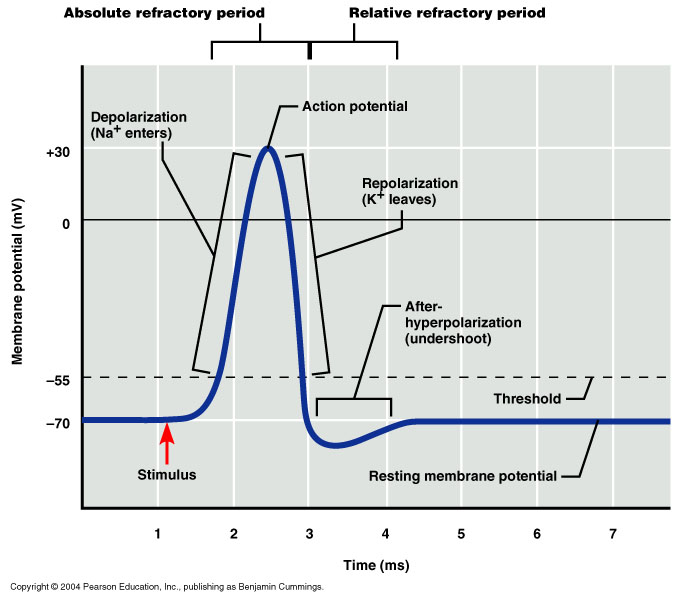
\includegraphics[width=0.7\textwidth]{images/actionpotential.jpg}
\caption{Schematic action potential and its main characteristics}
\label{fig:actionpotential}
\end{figure}

